\documentclass{article}

\usepackage{fancyhdr}
\usepackage{extramarks}
\usepackage{amsmath}
\usepackage{minted}
\usepackage{amsthm}
\usepackage{amsfonts}
\usepackage{tikz}
\usepackage[plain]{algorithm}
\usepackage{algpseudocode}

\usetikzlibrary{automata,positioning}
\usepackage{fullpage,enumitem,amsmath,amssymb,graphicx}

%
% Basic Document Settings
%

\topmargin=-0.75in
\textwidth=6.5in
\textheight=9.0in
\headsep=0.20in
\headheight = 12pt
\linespread{1.1}

\pagestyle{fancy}
\chead{\hmwkClass\ (\hmwkClassInstructor): \hmwkTitle}
\rhead{\firstxmark}
\lfoot{\lastxmark}
\cfoot{\thepage}

\renewcommand\headrulewidth{0.55pt}
\renewcommand\footrulewidth{0.55pt}

\setlength\parindent{0pt}


\setcounter{secnumdepth}{0}

%
% Homework Problem Environment
%
% This environment takes an optional argument. When given, it will adjust the
% problem counter. This is useful for when the problems given for your
% assignment aren't sequential. See the last 3 problems of this template for an
% example.

%
% Homework Details
%   - Title
%   - Due date
%   - Class
%   - Section/Time
%   - Instructor
%   - Author
%

\newcommand{\hmwkTitle}{Homework\ \#2}
\newcommand{\hmwkDueDate}{September 13, 2021}
\newcommand{\hmwkClassCode}{COT 5615}
\newcommand{\hmwkClass}{Math for Intelligent Systems}
\newcommand{\hmwkClassYear}{Fall 2021}
\newcommand{\hmwkClassInstructor}{Professor Kejun Huang}
\newcommand{\hmwkAuthorName}{\textit{Vyom Pathak}}
\newcommand{\hmwkUFID}{96703101}

%
%
%
% Various Helper Commands
%

% Useful for algorithms
\newcommand{\alg}[1]{\textsc{\bfseries \footnotesize #1}}

% For derivatives
\newcommand{\deriv}[1]{\frac{\mathrm{d}}{\mathrm{d}x} (#1)}

% For partial derivatives
\newcommand{\pderiv}[2]{\frac{\partial}{\partial #1} (#2)}

% Integral dx
\newcommand{\dx}{\mathrm{d}x}

% Alias for the Solution section header
\newcommand{\solution}{\textbf{\large Solution}}

% Probability commands: Expectation, Variance, Covariance, Bias
\newcommand{\E}{\mathrm{E}}
\newcommand{\Var}{\mathrm{Var}}
\newcommand{\Cov}{\mathrm{Cov}}
\newcommand{\Bias}{\mathrm{Bias}}

% norm bars
\newcommand{\norm}[1]{\left\lVert#1\right\rVert}

\begin{document}

\begin{center}
{\Large \hmwkClassCode\ \hmwkClass\ \hmwkClassYear\ \hmwkTitle}

\begin{tabular}{rl}
UFID: & \hmwkUFID \\
Name: & \hmwkAuthorName \\
Instructor: & \hmwkClassInstructor \\
Due Date: & \hmwkDueDate \\ 
% Collaborators: & [list all the people you worked with]
\end{tabular}
\end{center}

\section*{Problem 3.2}
\subsection*{RMS value and average of block vectors}
\subsubsection*{Solution}
Vector $x$ can be shown as follows: $x = (a_1,\ldots,a_n,b_1,\ldots,b_m)$
\begin{enumerate}[label=(\alph*)]
\item RMS of vector $x$ is:
\begin{align*}
\begin{split}
            rms(x) & = \sqrt{\frac{a_1^2+\ldots+a_n^2+b_1^2+\ldots+b_m^2}{n+m}}\\
            & = \sqrt{\frac{\frac{n(a_1^2+\ldots+a_n^2)}{n}+\frac{m(b_1^2+\ldots+b_m^2)}{m}}{n+m}}\\
            & = \sqrt{\frac{n\ rms(a)^2+m\ rms(b)^2}{n+m}}
\end{split}
\end{align*}
\item The average of vector $x$ is:
\begin{align*}
\begin{split}
    avg(x) & = \frac{a_1+\ldots+a_n+b_1+\ldots+b_m}{n+m}\\ 
    & = \frac{\frac{n(a_1+\ldots+a_n)}{n}+\frac{m(b_1+\ldots+b_m)}{m}}{n+m}\\
    & = \frac{n\ avg(a)+m\ avg(b)}{n+m}
\end{split}
\end{align*}
\end{enumerate}
\section*{Problem 3.5}
\subsection*{General norms}
\subsubsection*{Solution}
For 1-norm
\begin{enumerate}[label=(\alph*)]
  \item Homogeneity:
  \begin{align*}
  \begin{split}
      \norm{\beta x}_1 & = |\beta x_1| + |\beta x_1| + \ldots + |\beta x_n|\\
      & = |\beta|\ |x_1| + |\beta|\ |x_1| + \ldots + |\beta|\ |x_n|\\
      & = |\beta| (|x_1| + |x_1| + \ldots + |x_n|)\\
      & = |\beta| \norm{x}_1\\
  \end{split}
  \end{align*}
  \item Triangle inequality:
  \begin{align*}
  \begin{split}
      \norm{x + y}_1 & = |x_1+y_1| + |x_2+y_2| + \ldots + |x_n+y_n|\\
      & \leq |x_1| + |x_2| + \ldots + |x_n| + |y_1| + |y_2| + \ldots + |y_n|\\
      & = \norm{x}_1 + \norm{y}_1\\
  \end{split}
  \end{align*}
  \item Nonnegativity: Each term in $ \norm{x}_1 = |x_1| + |x_2| + \ldots + |x_n| $ is nonnegative.
  \item Definiteness: $\norm{x}_1$ = 0 only if $|x_1| = \ldots =  |x_n| = 0$
\end{enumerate}
For $\infty$-norm
\begin{enumerate}[label=(\alph*)]
    \item Homogeneity:
    \begin{align*}
        \begin{split}
            \norm{\beta x}_\infty & = max\{|\beta x_1|,|\beta x_2|,\ldots,|\beta x_n|\}\\
            & = max\{|\beta|\ |x_1|,|\beta|\ |x_2|,\ldots,|\beta|\ |x_n|\}\\
            & = |\beta|max\{|x_1|,|x_2|,\ldots,|x_n|\}\\
            & = |\beta|\norm{x}_\infty
        \end{split}
    \end{align*}
    \item Triangle inequality:
    \begin{align*}
        \begin{split}
            \norm{x + y}_\infty & = max\{|x_1+y_1| , |x_2+y_2| , \ldots , |x_n+y_n|\}\\
            & \leq max\{|x_1| + |y_1| ,|x_2| + |y_2|,  \ldots , |x_n| + |y_n|\}\\
            & \leq max\{|x_1|,|x_2|,\ldots,|x_n|\} + max\{|y_1|,|y_2|,\ldots,|y_n|\}\\
            & = \norm{x}_\infty + \norm{y}_\infty\\
        \end{split}
    \end{align*}
    \item Nonnegativity: According to it's definition, $\norm{x}_\infty$ is the largest of n nonnegative numbers $|x_j|$.
    \item Definiteness: $\norm{x}_\infty = 0$ only if $|x_j| = 0$ for $j = 1,\ldots,n$
\end{enumerate}
\section*{Problem 3.16}
\subsection*{Effect of scaling and offset on average and standard deviation}
\subsubsection*{Solution}
  \begin{enumerate}[label=(\alph*)]
      \item Finding $avg(\alpha x + \beta)$ as follows:
      \begin{align*}
    \begin{split}
        avg(\alpha x + \beta) & = \frac{1^T(\alpha x + \beta 1)}{n}\\
        & = \frac{\alpha 1^T x + \beta 1^T 1}{n}\\
        & = \alpha avg(x) + \beta\ \ (\because 1^T1 = n)
    \end{split}
      \end{align*}
    \item Finding $std(\alpha x + \beta)$ using (a) as follows:
    \begin{align*}
    \begin{split}
        std(\alpha x + \beta) & = rms(\alpha x + \beta - (\alpha avg(x) + \beta)1)\\
        & = rms(\alpha x - \alpha avg(x)1)\\
        & = |\alpha|rms(x-avg(x)1)\\
        & = |\alpha|std(x)
    \end{split}
    \end{align*}
  \end{enumerate}
\section*{Problem 3.26}
\subsection*{Time series auto-correlation}
\subsubsection*{Solution}
\begin{enumerate}[label=(\alph*)]
\item R(0) is the correlation coefficient between x and x with no lag and thus, it is always 1. For R($\tau$), with de-mean values as follows $(0_\tau,x-\mu1)$ and $(x-\mu1,0_\tau)$ and having the same norm $\norm{x-\mu1}$; their correlation coefficient is calculated as follows:
\begin{align*}
    R(\tau) = \frac{(0_\tau,x-\mu1^T)(x-\mu1,0_\tau)}{\norm{x-\mu1}^2}
\end{align*}
For $\tau \geq T$, the inner product in the numerator is 0 as for each jth vector-pair, one of the two vector has a 0 entry.
\item We can express $R(\tau)$ as follows:
\begin{align*}
\begin{split}
 R(\tau) & = \left(\frac{(0_\tau,x-\mu1)}{\norm{x-\mu1}}\right)^T\left(\frac{(x-\mu1,0_\tau)}{\norm{x-\mu1}}\right)\\
 & = \left(\frac{(0_\tau,x-\mu1)}{\sqrt{T}std(x)}\right)^T\left(\frac{(x-\mu1,0_\tau)}{\sqrt{T}std(x)}\right)\\
 & = \frac{1}{T} (0_\tau,z)^T(z,0_\tau)
\end{split}
\end{align*}
Here, according to (a) $R(\tau)=0$ for $\tau \geq T$ and thus the above equation for the remaining indices is given as follows:
\begin{align*}
    R(\tau) = \frac{1}{T}\sum\limits_{t=1}^{T-\tau}z_tz_{t+\tau}
\end{align*}
\item The series $x = (+1,-1,+1,-1,\ldots,+1,-1)$ has mean zero and norm $\sqrt{T}$. The auto-correlation can be calculated as follows:
\begin{align*}
    \begin{split}
        R(\tau) & = \frac{1}{T}\sum\limits_{t=1}^{T-\tau}x_tx_{t+\tau}\\
        & = \frac{1}{T}\sum\limits_{t=1}^{T-\tau}(-1)^{t+1}(-1)^{t+\tau+1}\\
        & = \frac{T-\tau}{T}(-1)^{\tau}\\
    \end{split}
\end{align*}
\item R(7) being high means that $z_t$ and $z_{t+7}$ are either higher than or lower than the mean value together. For examples, as $x_{t+7}$ is the number of meals served 7 days after $x_{t}$; number meals on Mondays are higher than the mean value and the number of meals are lower than the mean value on Saturdays. (Considering week starting from Saturday).  
\end{enumerate}
\section*{Problem A3.2}
\subsection*{Nearest neighbor and smallest angle}
\subsubsection*{Solution}

  \begin{minted}[
frame=lines,
framesep=2mm,
baselinestretch=1.2,
fontsize=\footnotesize,
linenos
]{julia}
using LinearAlgebra
a=[1,3,4]
xn = [[4,3,5],[0.4,10,50],[1,4,10],[30,40,50]]
dist = []
angle = []
for i in 1:4
    ntp = norm(a-xn[i])
    # println("Distance of a from x$i $ntp")
    push!(dist, ntp)
end
println("Minimum distance from a to x1,...,x4 is ",string(minimum(dist)))
for i in 1:4
    atp = acos((a'xn[i])/(norm(a)*norm(xn[i])))
    # println("Angle between a and x$i $atp")
    push!(angle, atp)
end
println("Minimum angle between a and x1,...,x4 is ",string(minimum(angle)))
\end{minted}
\section*{Problem A3.5}
\subsubsection*{Solution}
The $\norm{\alpha a + \beta b + \gamma c}$ can be solved as follows:
\begin{align*}
\begin{split}
\norm{\alpha a + \beta b + \gamma c}^2 & = (\alpha a + \beta b + \gamma c)^T(\alpha a + \beta b + \gamma c)\\
& = \alpha^2 a^Ta + \alpha\beta a^Tb + \alpha\gamma a^Tc + \beta\alpha b^Ta + \beta^2 b^Tb + \beta\gamma b^Tc + \gamma\alpha c^Ta + \gamma\beta c^Tb + \gamma^2 c^Tc\\
& = \alpha^2 \norm{a}^2 + \beta^2 \norm{b}^2 + \gamma^2 \norm{c}^2
(\because\ inner\ product\ of\ orthogonal\ vectors\ is\ 0.)\\
\end{split}
\end{align*}
\begin{align*}
    \therefore \norm{\alpha a + \beta b + \gamma c} = \sqrt{\alpha^2 \norm{a}^2 + \beta^2 \norm{b}^2 + \gamma^2 \norm{c}^2}
\end{align*}
\section*{Problem A4.2}
\subsection*{Topic discovery via k-means}
\subsubsection*{Solution}
\begin{enumerate}[label=(\alph*)]
    \item Following is the code:
\begin{minted}[
frame=lines,
framesep=2mm,
baselinestretch=1.2,
fontsize=\footnotesize,
linenos
]{julia}
include("wikipedia_corpus.jl")
include("kmeans.jl")
using Statistics
using LinearAlgebra
using SparseArrays
using Plots
pyplot()
#k=2
centroids, labels, j_hist = Kmeans.kmeans(article_histograms, 2);
centroids_2, labels_2, j_hist_2 = Kmeans.kmeans(article_histograms, 2);
itr1 = []
itr2 = []
for i in 1:length(j_hist)
    push!(itr1,i) 
end
for i in 1:length(j_hist_2)
    push!(itr2,i) 
end
plot(j_hist,itr1,label="Iteration 1",title="2 Centroids")
plot!(j_hist_2,itr2,label="Iteration 2")
#k=5
centroids, labels, j_hist = Kmeans.kmeans(article_histograms, 5);
centroids_2, labels_2, j_hist_2 = Kmeans.kmeans(article_histograms, 5);
itr1 = []
itr2 = []
for i in 1:length(j_hist)
    push!(itr1,i) 
end
for i in 1:length(j_hist_2)
    push!(itr2,i) 
end
plot(j_hist,itr1,label="Iteration 1",title="5 Centroids")
plot!(j_hist_2,itr2,label="Iteration 2")
#k=10
centroids, labels, j_hist = Kmeans.kmeans(article_histograms, 10);
centroids_2, labels_2, j_hist_2 = Kmeans.kmeans(article_histograms, 10);
itr1 = []
itr2 = []
for i in 1:length(j_hist)
    push!(itr1,i) 
end
for i in 1:length(j_hist_2)
    push!(itr2,i) 
end
plot(j_hist,itr1,label="Iteration 1",title="10 Centroids")
plot!(j_hist_2,itr2,label="Iteration 2")
\end{minted}
\begin{figure}[htp]

\centering
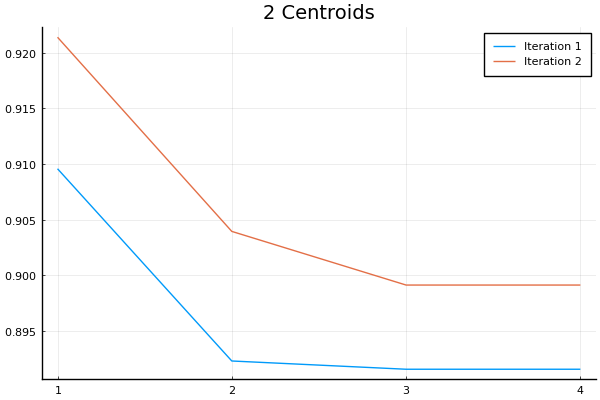
\includegraphics[width=.3\textwidth]{2-centroids.png}\hfill
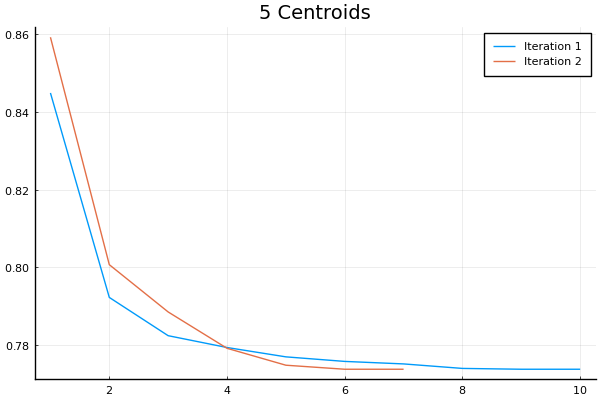
\includegraphics[width=.3\textwidth]{5-centroids.png}\hfill
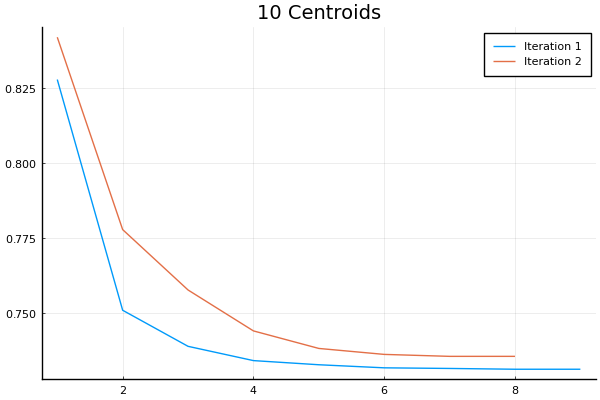
\includegraphics[width=.3\textwidth]{10-centroids.png}
\caption{Loss v/s Iterations Graphs for K = 2,5,10}
\label{fig:figure3}
\end{figure}
As I increased the number of centroids, the overall loss kept decreasing which indicates that there are at least 10 classes for the Wikipedia Article Corpus. Also, the loss is decreasing in similar manner even when the experiment is done twice for a single K-value.
\item Table~\ref{tab:my_label} describes the details learned by each topic and the three most common words for each topic as well. I used k=10 as the number of clusters.
\begin{table}[ht]
    \centering
    \begin{tabular}{p{0.7cm}p{5cm}p{9cm}}
    \hline
        Topic & 3 Most Common Words & Description  \\
    \hline
        1 & light,solar,sun & This topic is about radiation, Sun light, and mostly related to effect of sun light and other articles related to sun. It also contains articles on different effects of sun.\\
    \hline
    2 & painting,art,paintings & This topic is about different painters and different types of art and paintings. It also shows different types of painting styles in french.\\
    \hline
    3 & international,convention,member & This topic is about organizations, politics and different governing bodies. It encompasses different international organizations related to finances and other socioeconomic matters.\\
    \hline
    4 & signal,digital,telephone & This topic is about waves, signals and more specifically telephonic waves and its applications. It also explains wide variety of protocols related to telephonic and communication equipment.\\
    \hline
    5 & nations,council,general & This topic attributes about the national and international people, food-fodder and refugee committees. . It contains articles on world food orders, world peace meets, and other organizations which maintain balance between mankind throughout the world.\\
    \hline
    6 & weather,pressure,air & This topic is about effects and phenomenon related to weather, and other instruments used to measure them. It also contains articles on weather maps,and weather modifications.\\
    \hline
    7 & radio,signal,frequency & This topic is about signals and phenomenons related to signals and radio waves. It also contains articles on different effects and types of waves.\\
    \hline
    8 & pokemon,game,games & This topic is about Pokemon's; their types and different names and their details.\\
    \hline
    9 & ice,rain,freezing & This topic is about different types of ice and ice related weather events and other ice phenomenons.\\
    \hline
    10 & wind,temperature,humidity & This topic is about wind and different equipment's as well as terms related to the study of wind and temperature. \\
    \hline
    \end{tabular}
    \caption{Topic details for 10-Clusters on Wikipedia Article Corpus}
    \label{tab:my_label}
\end{table}
Code used to generate the data and analyze it:
\begin{minted}[
frame=lines,
framesep=2mm,
baselinestretch=1.2,
fontsize=\footnotesize,
linenos
]{julia}
open("Cluster_Data.txt", "w") do file
    for i in 1:10
        topic = "Topic Number: "*string(i)
        titles = article_titles[labels_2 .== i]
        words = dictionary[sortperm(centroids_2[i],rev=true)]
        ans = topic*"\nTitles: "*join(titles,",")*" \nCommon Words: "*join(words,",")*"\n\n"
        write(file, ans)
    end
end
\end{minted}
\end{enumerate}
\end{document}
